\stepcounter{subsection}
\subsection{}

\begin{figure}[H]
     \centering
     \begin{subfigure}{0.3\textwidth}
         \centering
         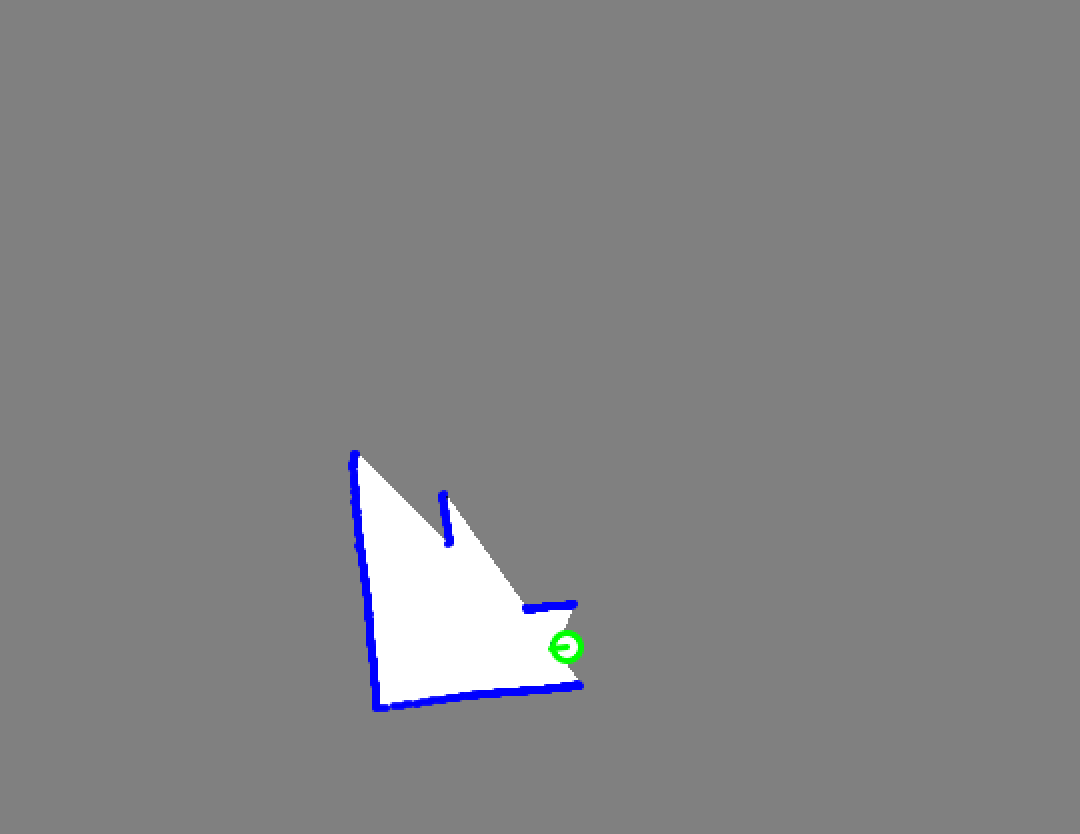
\includegraphics[width=\textwidth]{figures/mapping_2s.png}
         \caption{$t = \SI{2}{\second}$}
         \label{mapping2s}
     \end{subfigure}
     \hfill
     \begin{subfigure}{0.3\textwidth}
         \centering
         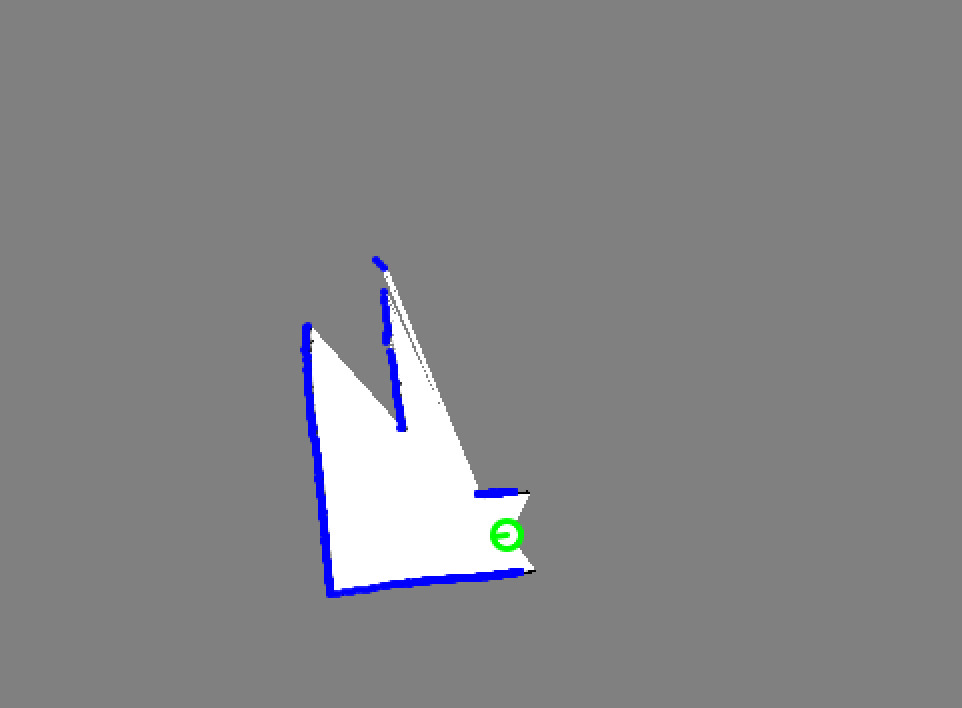
\includegraphics[width=\textwidth]{figures/mapping_8s.png}
         \caption{$t = \SI{8}{\second}$}
         \label{mapping8s}
     \end{subfigure}
     \hfill
     \begin{subfigure}{0.3\textwidth}
         \centering
         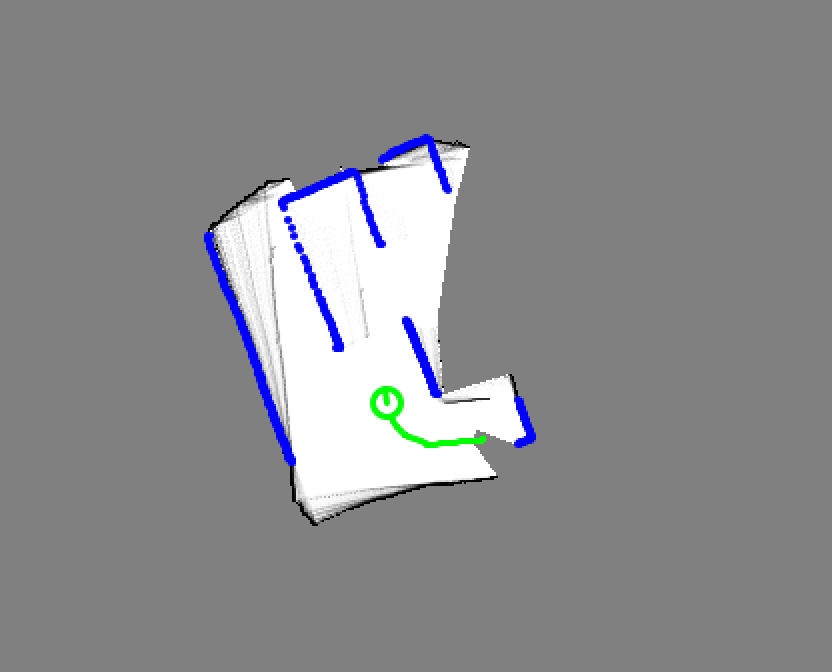
\includegraphics[width=\textwidth]{figures/mapping_20s.png}
         \caption{$t = \SI{20}{\second}$}
         \label{mapping20s}
     \end{subfigure}
        \caption{Mapping}
        \label{fig:three graphs}
\end{figure}

\subsection{}

The localization uses the current roboter pose in the map. Errors in the roboter pose are directly reflected in the map because the obstacles are drawn relative to the roboter pose. Therefore, it is important to have an accurate roboter pose which is not easy as there might be different error sources like slippage or inaccuracies in the robots movement. To improve this, one should do simultanious localization and mapping to increase the accuracy of the robot pose. 